\pagebreak
\section{ECCO Metadata Specification}
\subsection{Overview Description of the ECCO Metadata Model}
The GHRSST data are global collections compiled by scientists and data production systems in many
countries, so the ISO 19115-2 International Geographic Metadata Standard (extensions for imagery
and gridded data) has been adopted as the standard for GDS 2.0 metadata. This standard provides a
structured way to manage not just the data usage and granule-level discovery metadata provided by
the CF metadata in the GHRSST netCDF files, but also collection-level discovery, data quality,
lineage, and other information needed for long-term stewardship and necessary metadata
management. The GHRSST GDAC and LTSRF work with individual RDACs to create and maintain
the collection-level ISO record for each of their datasets (one collection level record for each product
line). The collection level record will be combined by the GDAC with metadata embedded in the
netCDF-4 files preferred by the GDS 2.0. In the event that an RDAC chooses to produce netCDF-3
files instead of netCDF-4, they must also create a separate XML metadata record for each granule
(following the GDS 1.6 specification detail in [RD-1]). RDACs will assist with maintaining the collection
portion of the ISO metadata record and will update it on an as-needed basis. This approach ensures
that for every L2P, L3, L4, or GMPE granule that is generated, appropriate ISO metadata can be
registered at the GHRSST Master Metadata Repository (MMR) system. Details of this approach are
provided in Section 13.3 after a brief description of the heritage GDS 1.0 metadata approach.
\par

\subsection{Evolution from the GHRSST GDS 1.0 Metadata Model}
The GDS 1.6 specification metadata model ([RD-1]) contained three distinct metadata records. The
Data Set Descriptions (DSD) included metadata that provided an overall description of a GHRSST
product, including discovery and distribution. These metadata changed infrequently and were termed
collection level metadata. The File Records (FR) contained metadata that describe a single data file
or granule (traditionally called granule metadata). Finally there was also granule metadata captured in
the CF attributes of a netCDF3 file. Under the new GDS 2.0 initial GHRSST 2.0 Metadata Model, all
three types of metadata are leveraged into a single ISO-compliant metadata file as shown in Figure
13-2. Future revisions of the GDS 2.0 will incorporate more of the ISO metadata capabilities.
\par

\subsection{The ISO 19115-2 Metadata Model}
The ISO metadata model is made up of a set of containers (also referred to as classes or objects)
that contain metadata elements or other objects that, in turn, contain other elements or objects (see
Figure 13-1 and Table 13-1). The root element is MI\_Metadata1 \footnotemark{}
. It contains twelve major classes that document
various aspects of the resource (series or dataset) being described. The MD\_DataIdentification object
contains other major classes that also describe various aspects of the dataset.
\newp \footnotetext{The ISO Standard for Geographic Data has two parts. ISO 19115 is the base standard. ISO 19115-2 includes 19115 and
adds extensions for images and gridded data. We will use both parts in this model and refer to the standard used as 19115-2.}

\begin{figure}[H]
\centering
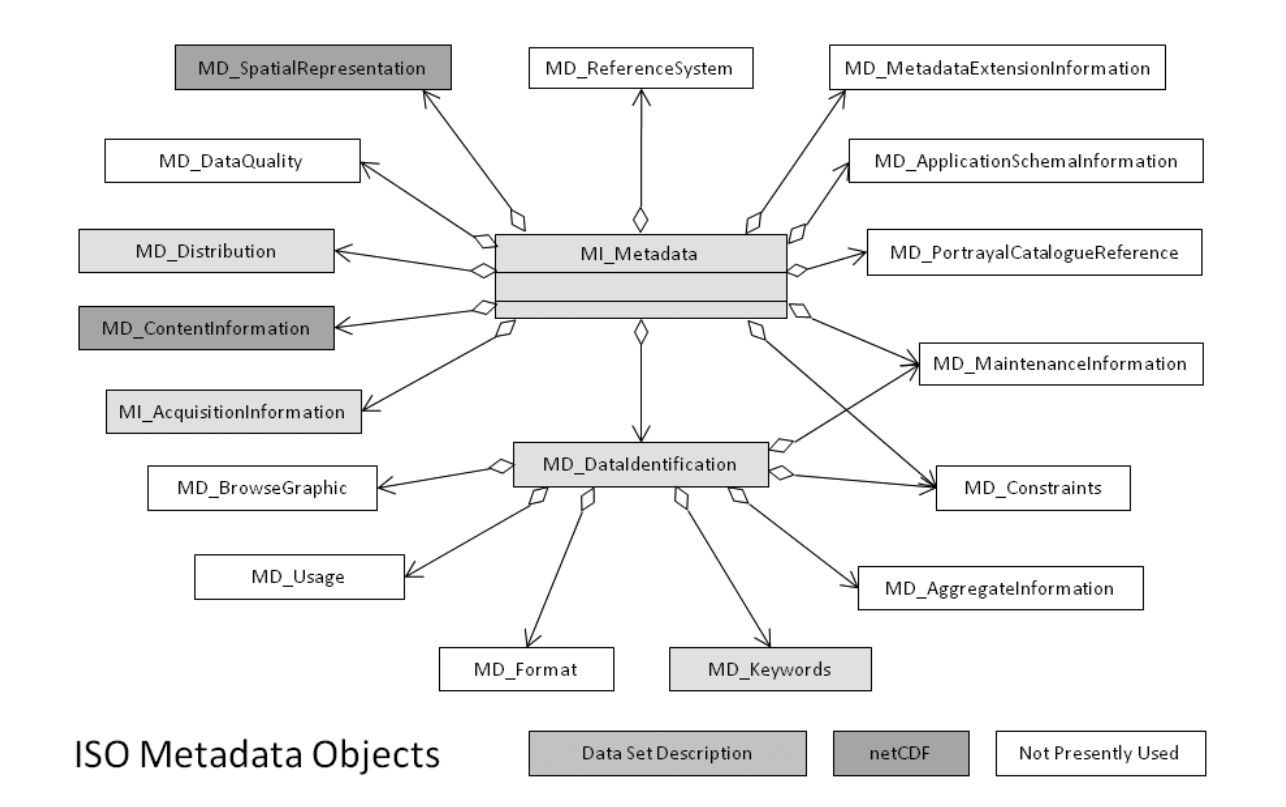
\includegraphics[width=0.7\textwidth]{../images/iso_metadata_obj.png}
\caption{ISO Metadata Objects and their sources}
\label{fig:ISO_Metadata_Objects}
\end{figure}

\begin{longtable}{|p{0.4\textwidth}|p{0.6\textwidth}|}
    \caption{Major ISO Objects. Objects in use in the GHRSST metadata model are shaded in
gray.}
    \label{tab:table-major_iso_objects} \\
    \hline \endhead \hline \endfoot
    \textbf{ISO Object} & \textbf{Explanation} \\ \hline
    \rowcolor{lightgray} MI\_Metadata & Root element that contains information about the metadata itself. \\ \hline 
    \rowcolor{lightgray} MI\_AcquisitionInformation & Information about instruments, platforms, operations and other element of data acquisition. \\ \hline 
    \rowcolor{lightgray} MD\_ContentInformation & Information about the physical parameters and other attributes contained in a resource. \\ \hline
    \rowcolor{lightgray} MD\_Distribution & Information about who makes a resource available and how to get it. \\ \hline 
    \rowcolor{lightgray} MD\_DataQuality & Information about the quality and lineage of a resource. \\ \hline 
    \rowcolor{lightgray} MD\_SpatialRepresentation & Information about the geospatial representation of a resource. \\ \hline
    \rowcolor{lightgray} MD\_ReferenceSystem & Information about the spatial and temporal reference systems used in the resource. \\ \hline
    MD\_MetadataExtensionInformation  & Information about user specified extensions to the metadata standard used to describe the resource. \\ \hline
    MD\_ApplicationSchemaInformation & Information about the application schema used to build a dataset (not presently used for GHRSST metadata). \\ \hline 
    MD\_PortrayalCatalogueReference & Information identifying portrayal catalogues used for the resource (not presently used for GHRSST metadata). \\ \hline
    MD\_MaintenanceInformation & Information about maintenance of the metadata and the resource it describes. \\ \hline
    \rowcolor{lightgray}MD\_Constraints & Information about constraints on the use of the metadata and the resource it describes. \\ \hline
    \rowcolor{lightgray}MD\_DataIdentification & Information about constraints on the use of the metadata and the resource it describes. \\ \hline
    \rowcolor{lightgray}MD\_AggregateInformation & Information about groups that the resource belongs to.\\ \hline
    \rowcolor{lightgray}MD\_Keywords & Information about discipline, themes, locations, and times included in the resource. \\ \hline
    \rowcolor{lightgray} MD\_Format & Information about formats that the resource is available in. \\ \hline
    MD\_Usage & Information about how the resource has been used and identified limitations. \\ \hline
    MD\_BrowseGraphic  & Information about graphical representations of the resource. \\ 
\end{longtable}

MI\_Metadata objects can be aggregated into several kinds of series that include metadata describing
particular elements of the series, termed dataset metadata, as well as metadata describing the entire
series (i.e. series or collection metadata). Unlike the GDS 1.0 Metadata Model, the ISO-based GDS
2.0 model combines both collection level and granule level metadata into a single XML file. The initial
approach will be to extract and translate granule metadata from netCDF-4 CF attributes in conjunction
with collection level metadata from existing GDS 1.0 compliant DSD records. In the case of a data
producer providing a netCDF-3 granule, an additional FR metadata record \textbf{must} still be provided (see
GDS 1.6 for details on the format of the FR metadata records). The flow of metadata production is
described below in two scenarios:
\newp

Existing GDS 1.0 GHRSST products
\setlist{nolistsep}
\begin{enumerate}[noitemsep]
    \item Generate ISO collection level metadata from existing GDS 1.0 DSD records
    \item Generate ISO granule level metadata from CF attributes embedded in a GDS 2.0 specification netCDF4 granule
    \item Combine 1 and 2 into a complete GDS 2.0 ISO 19115-2 record
    \item If the granule is GDS 1.0 netCDF3 format the RDAC must provide a File Record 
\end{enumerate}
\newp

GDS 2.0 GHRSST products
\setlist{nolistsep}
\begin{enumerate}[noitemsep]
    \item Use existing ISO collection level metadata. RDACs will provide the initial metadata record from a template.
    \item Generate ISO granule level metadata from CF attributes embedded in a GDS 2.0 specification netCDF4 granule
    \item Combine 1 and 2 into a complete GDS 2.0 ISO 19115-2 record 
\end{enumerate}
\newp

In both cases, the GDAC has the primary role to create the ISO metadata records in steps 1-3. A
RDAC can also choose to do steps 1-3, or maintain only the collection level portion.
\newp

A diagram of the production approach is shown in Figure 13-2. The root element for the combined file
is DS\_Series which includes dataset and series metadata. Dataset metadata will be constructed
using metadata extracted from the netCDF-4 CF attributes (or a FR record if the file is in netCDF3
format). Series Metadata will be constructed with information from (initially) the DSD or the collection
level portion of an existing GDS 2.0 specification ISO record.
\newp 

\begin{figure}[H]
\centering
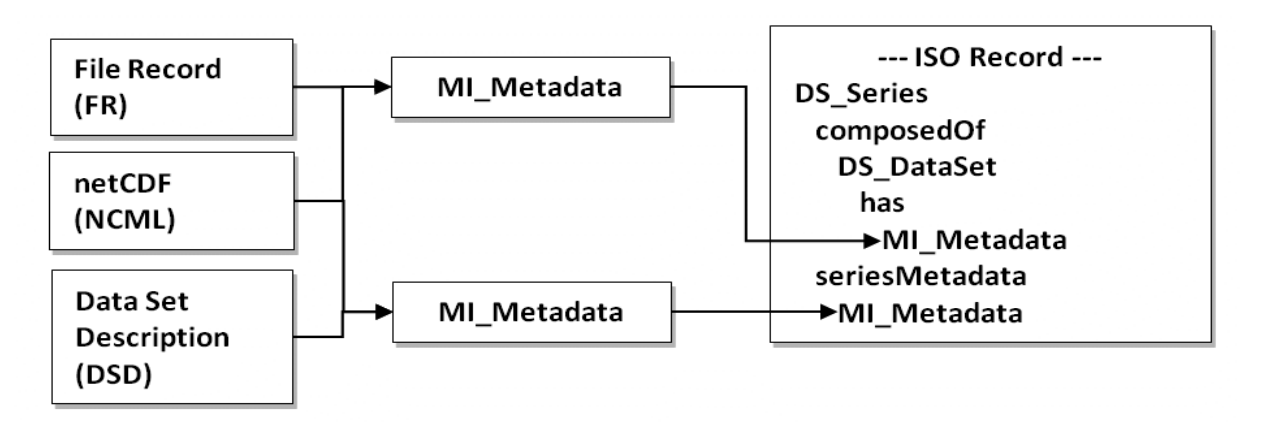
\includegraphics[width=0.9\textwidth]{../images/ghrsst_metadata_translation.png}
\caption{Initial GHRSST Metadata Translation Approach to ISO record}
\label{fig:GHRSST_metadata_translation}
\end{figure}

To see the comprehensive details of the GHRSST GDS 2.0 metadata model refer to the GDS 2.0
Metadata Specification documents and example at the GDAC (\url{http://ghrsst.jpl.nasa.gov}).